%\pagestyle{myheadings}
%\markright{{\large ME 4140 Fall 2020---The Robotic Operating System}}

% Tennessee Technological University
% ME4140 - Fall 2016 - Fall 2017 - Fall 2020 
% Tristan Hill - September 10, 2020
% Module 4 - Turtlebot Family

%\textwidth=6.5in
%\topmargin=-0.5in
%\textheight=9.25in
%\hoffset=-0.5in
%\footskip=0.2in


\documentclass[fleqn]{beamer}                         % for presentation (has nav buttons at bottom)
%\documentclass[handout]{beamer}  % for handout 
\usepackage{beamerthemesplit}
\usepackage{amsmath}
\usepackage{listings}
\usepackage{multicol}
\usepackage{framed}
\usepackage{graphicx}
\usepackage{keystroke}

\usepackage{varwidth}
\usepackage{tasks}
\usepackage{fleqn}

\usepackage{minted}
\setminted[text]{
	escapeinside=||, 
	%breaksymbolleft=\carriagereturn,
	frame=single,
	%showspaces=true
	framesep=2mm,
	baselinestretch=1.2,
	bgcolor=mygray
}

%\textwidth=6.0in
%\topmargin=-0.6in
%\leftmargin=0.5in
%\textheight=9.25in
%\hoffset=-0.5in
%\footskip=0.2in

\beamertemplateballitem

% custom colors
\definecolor{TTUpurple}{rgb}{0.3098, 0.1607, 0.5176} % TTU Purple (primary)
\definecolor{TTUgold}{rgb}{1.0000, 0.8666, 0.0000} % TTU Gold (primary) 
\definecolor{mygray}{rgb}{.6, .6, .6}
\definecolor{mypurple}{rgb}{0.6,0.1961,0.8}
\definecolor{mybrown}{rgb}{0.5451,0.2706,0.0745}
\definecolor{mygreen}{rgb}{0, .39, 0}
\definecolor{mypink}{rgb}{0.9960, 0, 0.9960}

% color commands
\newcommand{\R}{\color{red}}
\newcommand{\B}{\color{blue}}
\newcommand{\BR}{\color{mybrown}}
\newcommand{\K}{\color{black}}
\newcommand{\G}{\color{mygreen}}
\newcommand{\PR}{\color{mypurple}}
\newcommand{\PN}{\color{mypink}}
\newcommand{\OR}{\color{TTU}}
\newcommand{\GD}{\color{TTUgold}}

% beamer colors
\setbeamercolor{palette primary}{bg=TTUpurple,fg=TTUgold}
\setbeamercolor{palette secondary}{bg=black,fg=TTUgold}
\setbeamercolor{palette tertiary}{bg=black,fg=TTUpurple}
\setbeamercolor{palette quaternary}{bg=TTUgold,fg=black}
\setbeamercolor{structure}{fg=TTUpurple} % itemize, enumerate, etc
\setbeamercolor{section in toc}{fg=TTUpurple} % TOC sections

\newcommand{\Lagr}{\mathcal{L}} % lagrangian

\newcommand{\hspcu}{\underline{\hspace{20mm}}} % large horizontal space w underline
\newcommand{\vspccc}{\vspace{6mm}\\} % large vertical space
\newcommand{\vspcc}{\vspace{4mm}\\}   % medium vertical space
\newcommand{\vspc}{\vspace{2mm}\\}     % small vertical space

\newcommand{\hspcccc}{\hspace{10mm}} % large horizontal space
\newcommand{\hspccc}{\hspace{6mm}} % large horizontal space
\newcommand{\hspcc}{\hspace{4mm}}   % medium horizontal space
\newcommand{\hspc}{\hspace{2mm}}     % small horizontal space

% windows logo
% Lower the picture a little to match the text baseline
\newcommand{\WindowsLogo}{\raisebox{-0.1em}{%
  
\includegraphics[height=0.8em]{win_logo}}}
\newcommand{\WinKey}{\keystroke{\WindowsLogo}}

\newcommand{\CTRL}{\raisebox{-0.1em}{Ctrl}}
\newcommand{\CTRLKey}{\keystroke{\CTRL}}

\newcommand{\ALT}{\raisebox{-0.1em}{Alt}}
\newcommand{\ALTKey}{\keystroke{\ALT}}

\newcommand{\pkgname}{\G<package\_name>\K}
\newcommand{\wspname}{\R<workspace\_name>\K}
\newcommand{\nodname}{\PR<node\_name>\K}
\newcommand{\tpcname}{/topic\_name}
\newcommand{\home}{\textasciitilde/}
\newcommand{\rosdistro}{kinetic}

\newsavebox{\mybox} % custom box

\newcommand{\MNUM}{4\hspace{2mm}} % Module number
\newcommand{\TNUM}{---\hspace{2mm}} % Topic number - single topic for now
\newcommand{\moduletitle}{Turtlebot Family} % Titles and Stuff
%\newcommand{\topictitle}{---} 

\newcommand{\sectiontitleI}{A Brief History} % More Titles and Stuff
\newcommand{\sectiontitleII}{Recent Models}
\newcommand{\sectiontitleIII}{Turtlebot3 at TNTECH}
\newcommand{\sectiontitleIV}{Tutorial 4 - Turtlebot3}

\title{ME4140 - ROS Workshop}

\author{Mechanical Engineering \vspc Tennessee Technological University}

\date{Tristan Hill, Lecturer}

\begin{document}

\lstset{language=MATLAB,basicstyle=\ttfamily\small,showstringspaces=false}

\frame{\titlepage \center\begin{framed}\Large \textbf{Module \MNUM - \moduletitle}\end{framed} \vspace{5mm}}

% Section 0 - Outline
\frame{
	
	\large \textbf{Module \MNUM - \moduletitle} \vspace{3mm}\\
	
	\begin{itemize}
	
		\item \hyperlink{sectionI}{\sectiontitleI}    \vspc % Section I
		\item \hyperlink{sectionII}{\sectiontitleII} 	\vspc % Section II
		\item \hyperlink{sectionIII}{\sectiontitleIII} 	\vspc %Section III
		\item \hyperlink{sectionIV}{\sectiontitleIV} \vspc %Section IV	
	
	\end{itemize}

}

\section{\sectiontitleI}

	% Section I - Frame I
	\frame[containsverbatim]{ \small
		\frametitle{\sectiontitleI}



}


	% Section I - Frame II
	\frame[containsverbatim]{ \small
		\frametitle{\sectiontitleI}

	}

\section{\sectiontitleII}

	% Section II - Frame I
	\frame[containsverbatim]{ \small
		\frametitle{\sectiontitleII}
		
  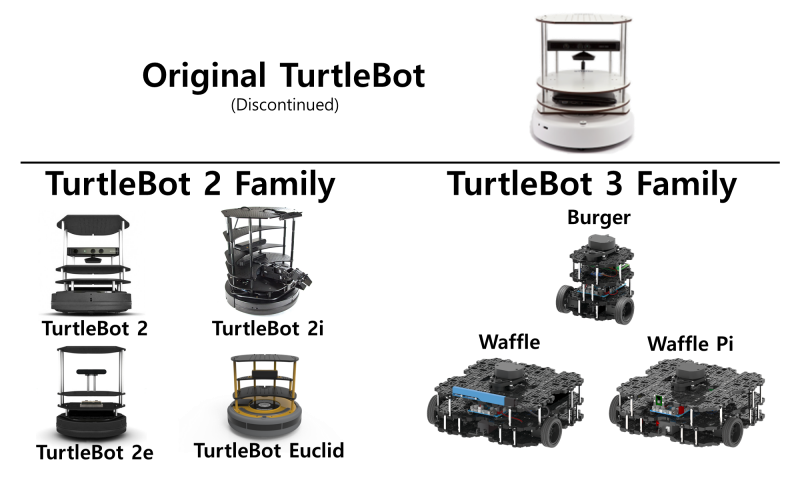
\includegraphics[scale=.35]{turtlebot_family.png}


}

\section{\sectiontitleIII}

	% Section II - Frame I
	\frame{ \small
		\frametitle{\sectiontitleIII}
	

}


\section{\sectiontitleIV}	
	% Section V - Frame I
	            \begin{frame}[label=sectionIV] \small
		\frametitle{\sectiontitleIV}    
	
 \setbeamertemplate{itemize items}[triangle]
                \begin{itemize}

					\item {\bf Overview:} Turtles are cool! Your next exercise is to setup your computer so that you can begin learning ROS. 		

					\item {\bf Assignment:} Complete the tutorial in the document {\it tutorial4\_turtlebot3\_simulator.pdf } on ilearn. You must be able to drive your turtlebot3 around the virtual arena.
                    
                    \item {\bf Deliverable:} Write a one to two paragraph summary of what you accomplished and what you struggled with the most. Include an image of the turtlesim window after you have driven a pattern. 
    
                    \item {\bf Next Week:} After completion of Module 3, you are ready for a better robot. You will learn to use a simulated turtlebot3 in a Gazebo simulator. \vspc
                    
       
                \end{itemize}
		\end{frame}

\end{document}


%
%\begin{description}
%
%    \item [I. Components] The major building blocks of a ROS system
%
%        \begin{enumerate}
%                
%            \item \href{http://wiki.ros.org/Master}{Master Node}
%                \begin{itemize}
%                    \item {\it The ROS Master provides naming and registration services to the rest of the nodes in the ROS system.}** 
%                    \item master node runs first  {\fontfamily{qcr}\selectfont  \hspace{5mm} \$ roscore } \\
%                    \item core of the system or robot {\fontfamily{qcr}\selectfont  \hspace{5mm} \$ ROS\_MASTER\_URI=http://12345 } \\
%                    
%
%                \end{itemize}
%            
%            \item \href{http://wiki.ros.org/Nodes}{Nodes}             
%                \begin{itemize}
%                    \item {\it A node is a process that performs computation.}** 
%                    \item each 'program' or 'element' of the robot is a node\\examples:
%                        \begin{itemize} 
%                        \begin{multicols}{2}    
%                        
%                            \item sensor
%                            \item hardware driver    
%                            \item navigation 
%                            \item keyboard or joystick        
%                            
%                        \end{multicols}
%                        \end{itemize}
%                    \item start or run node individually after master\vspace{5mm}\\
%                    {\fontfamily{qcr}\selectfont  \hspace{5mm} \$ rosrun <packagename> <nodename> <options> } \vspace{1mm}\\
%                  
%                    \item all nodes are registered to the master and communicate in different ways
%                        \begin{itemize}
%                            \item  \href{http://wiki.ros.org/Topics}{topics} - publishing and subscribing
%                            \item \href{http://wiki.ros.org/Parameter%20Serverparameters}{parameter server} - static data
%                            \item \href{http://wiki.ros.org/Services}{services} - subroutine call
%                        \end{itemize}    
%                                      
%                \end{itemize}
%                
%            \item \href{http://wiki.ros.org/Packages}{Packages} 
%
%                \begin{itemize}
%                    \item {\it Software in ROS is organized in packages. A package might contain ROS nodes, a ROS-independent library, a dataset, configuration files, a third-party piece of software, or anything else that logically constitutes a useful module.}** 
%                    \item a collection of related nodes, each node belongs to a package
%                                     
%                    \item pre-built packages available with ros installation {\fontfamily{qcr}\selectfont  \hspace{5mm} -desktop-full}
%                    \item pre-built packages available for installation \\
%                    \begin{description}
%                        \item[apt] {\fontfamily{qcr}\selectfont  \hspace{1mm} \$ sudo apt-get install ros-<distribution>-<packagename> } 
%                        \item[rosdep]{\fontfamily{qcr}\selectfont  \hspace{1mm} \$ rosdep install <packagename> } \\
%                    \end{description}
%                    \item update ubuntu before installing anything \\
%                    {\fontfamily{qcr}\selectfont  \hspace{2mm} \$ sudo apt-get update } \\
%                    {\fontfamily{qcr}\selectfont  \hspace{2mm} \$ sudo apt-get check }                
%                \end{itemize}            
%
%                
%                
%    \end{enumerate}
%    ** from (ros.org)
%    \newpage
%    
%    \item [II. The Graph of the System] ROS works on a system of interconnected nodes. It is very useful to visualize this in a graph.\\
%        \begin{enumerate}   
%            
%            \item \href{http://wiki.ros.org/rqt_graph}{RQT Graph} A very useful tool. A node {\it rqt\_graph} in a package {\it rqt\_graph}. \\\\
%                    {\fontfamily{qcr}\selectfont  \hspace{5mm} \$ rosrun rqt\_graph rqt\_graph}\\
%            
%            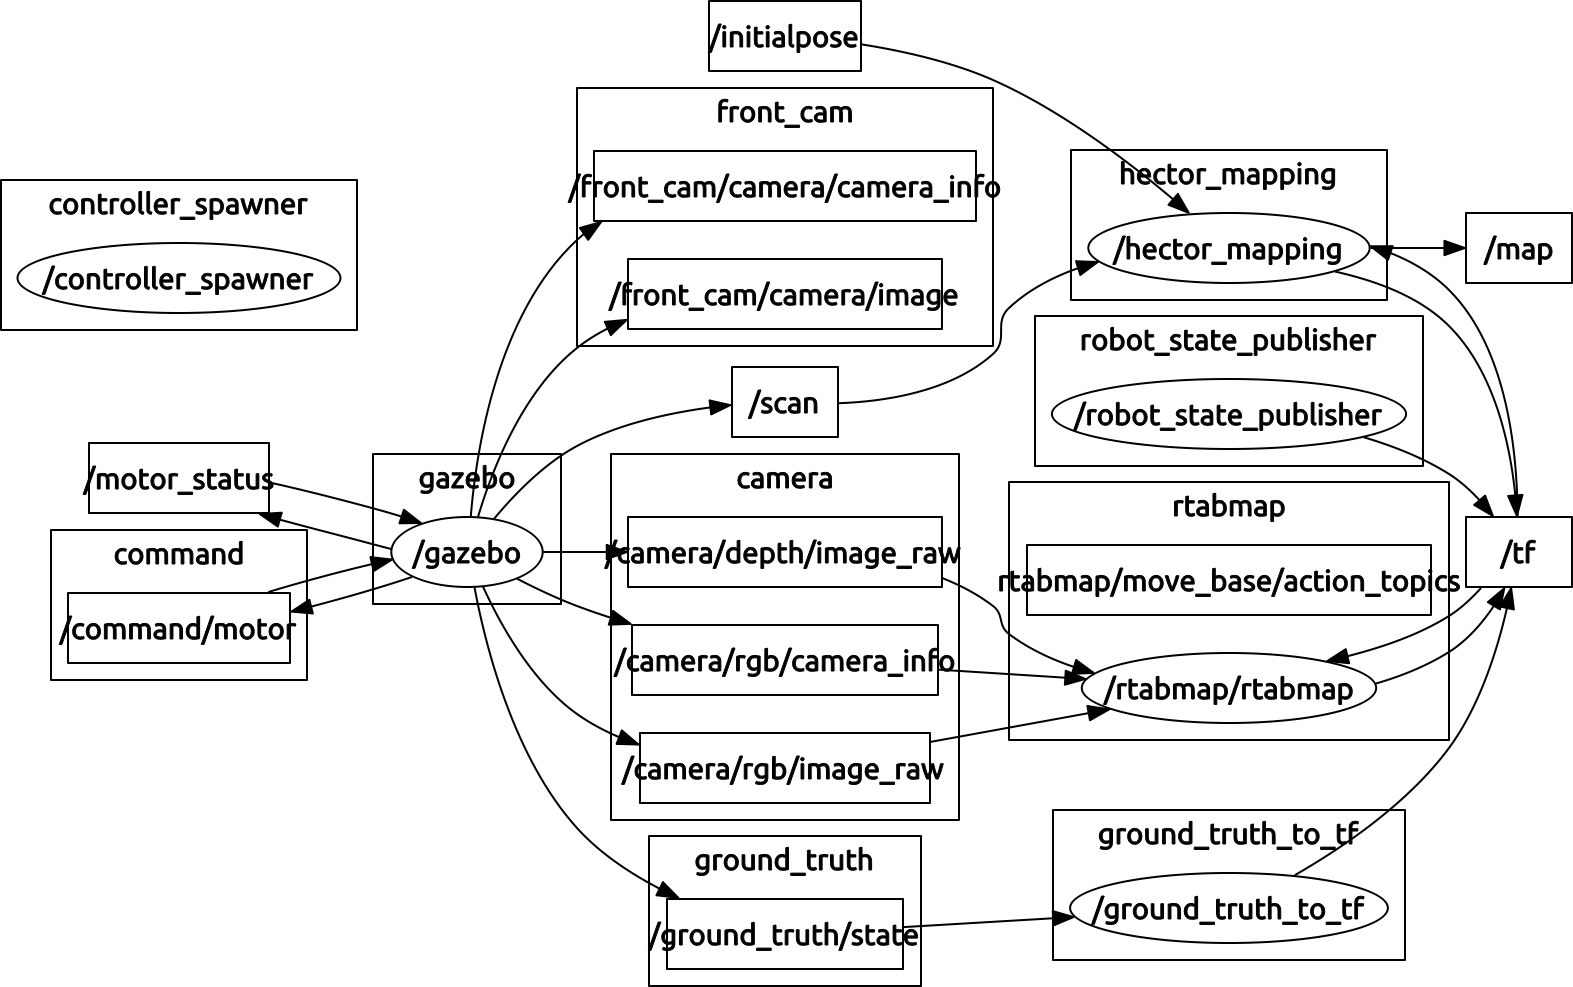
\includegraphics[scale=.4]{ros_basics_fig1.png} \\
%            
%            \item \href{http://wiki.ros.org/rqt_plot}{RQT Plot} A very useful tool. A node {\it rqt\_plot} in a package {\it rqt\_plot}. \\
%                {\fontfamily{qcr}\selectfont  \hspace{5mm} \$ rosrun rqt\_plot rqt\_plot}\\
%            
%            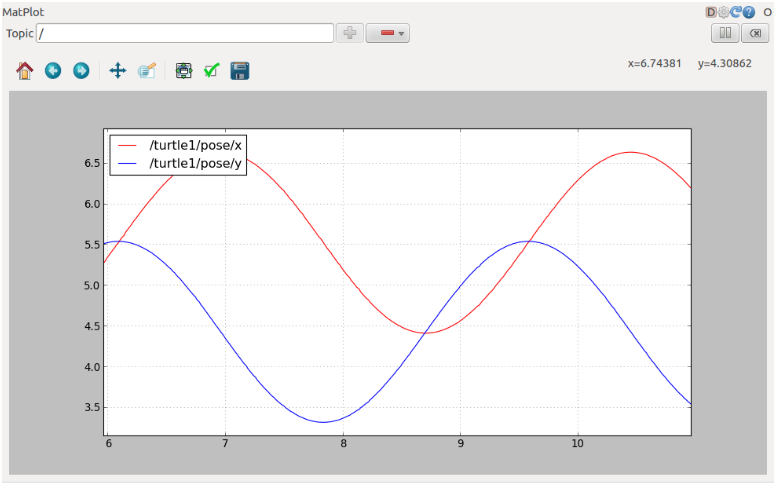
\includegraphics[scale=.5]{ros_basics_fig2.png} \\    
%          \end{enumerate}       
%
%
%\newpage
%    
%    \item [III. Topics, Publishers, and Subscribers] The nodes in a ROS system communicate.  
%        \begin{enumerate}   
%           \item \href{http://wiki.ros.org/Topics}{Topics} 
%                    \begin{itemize}
%                        \item data available to nodes in the system
%                        \item each topic has a name    
%                        \item data is stored and transferred in standard ros data types
%                        \item generally data is streaming, but does not have to be
%                    \end{itemize}    
%           \item \href{http://wiki.ros.org/ROS/Tutorials/WritingPublisherSubscriber(c++)}{Publishers}
%                    \begin{itemize}
%      
%                        \item data produced by a node can be shared with the system by publishing a topic
%                        \item a node which outputs topic data is a publisher
%                        \item a node may publish multiple topics 
%                        
%                        \end{itemize}  
%            \item \href{http://wiki.ros.org/ROS/Tutorials/WritingPublisherSubscriber(c++)}{Subscribers}
%                \begin{itemize}
%      
%                        \item a registered node can access the data in a topic by subscribing to a topic
%                        \item a node which gets topic data as input is a subscriber
%                        \item a node may subscribe to multiple topics 
%                    \end{itemize}  
%                    
%            \item \href{http://wiki.ros.org/rostopic}{rostopic}                    
%                \begin{itemize}   
%                    \item a very useful tool, a built in package 
%                    \item used differently than other packages, does not require rosrun
%                    \item a set of different tools
%                    \begin{description}   
%                        \item [list] {\fontfamily{qcr}\selectfont  \hspace{5mm} \$ rostopic list}\\
%                        \item [echo] {\fontfamily{qcr}\selectfont  \hspace{5mm} \$ rostopic echo /topicname}\\
%                        \item [type] {\fontfamily{qcr}\selectfont  \hspace{5mm} \$ rostopic pub /topicname}\\
%                    \end{description}  
%                \end{itemize}    
%                    \item  \href{http://wiki.ros.org/msg}{data types} - topics are published in standard types called messages
%                    \begin{itemize}
%                        \item {\fontfamily{qcr}\selectfont  \hspace{5mm} std\textunderscore msgs/int32 }
%                        \item {\fontfamily{qcr}\selectfont  \hspace{5mm} std\textunderscore msgs/float32 }\\
%                        
%                        \item {\fontfamily{qcr}\selectfont  \hspace{5mm} geometry\textunderscore msgs/Point }
%                        \item {\fontfamily{qcr}\selectfont  \hspace{5mm} geometry\textunderscore msgs/Pose }\\
%                        
%                        \item {\fontfamily{qcr}\selectfont  \hspace{5mm} nav\textunderscore msgs/Odometry }
%                        \item {\fontfamily{qcr}\selectfont  \hspace{5mm} nav\textunderscore msgs/Path }\\
%                    \end{itemize}
%                    
%                    \item let show an example now!
%                                      
%        \end{enumerate}     
%\newpage
%    
%%    \item [IV. Services] The nodes in a ROS system can also communicate through services. Thsi is for reply/request type operations.  
%%  \begin{enumerate} 
%%\item \href{http://wiki.ros.org/Services}{Services}
%%\end{enumerate}    
%%\newpage
%    
%
%\end{description}
%\end{document}
%
